\chapter{\IfLanguageName{dutch}{Stand van zaken}{State of the art}}%
\label{ch:stand-van-zaken}

% Tip: Begin elk hoofdstuk met een paragraaf inleiding die beschrijft hoe
% dit hoofdstuk past binnen het geheel van de bachelorproef. Geef in het
% bijzonder aan wat de link is met het vorige en volgende hoofdstuk.

% Pas na deze inleidende paragraaf komt de eerste sectiehoofding.

\section{Network and Information Security 2}%
\label{sec:nis2}

\section{Huidige aanpak van configuration management}%
\label{sec:huidige-aanpak-van-configuration-management}

In dit gedeelte wordt de huidige aanpak van configuration management besproken, met een focus op Infrastructure as Code (IaC).
Naast wat het is, wordt er ook gekeken naar de fundamentele componenten van IaC, alsook de voordelen ervan.
Ook zullen er tools vernoemd worden die we kunnen gebruiken om de configuratie van een systeem te ontdekken, om later om te zetten naar een IaC omgeving.

\subsection{Infrastructure as Code}%
\label{sub:iac}

Sinds de opkomst van computernetwerken is het uitrollen en beheren van servers en netwerken altijd een uitdagende taak geweest.
Infrastructure as Code (IaC) is een concept dat de laatste jaren steeds meer aan populariteit wint. Dit komt vooral doordat het beheerders van zulke netwerken in staat stelt om hun configuratie en infrastructuur vast te leggen in code, in plaats van handmatig te configureren.
Binnen deze code kunnen veelvoorkomende, complexe taken automatisch worden uitgevoerd, en dit alles op een geteste en foutloze manier~\autocite{chef-what-is-iac}.

IaC is gebaseerd op drie fundamentele concepten~\autocite{chef-what-is-iac}:
\begin{itemize}
    \item Automatisering: Het aanpassen van handmatige configuratie en het uitrollen van nieuwe servers worden allemaal geautomatiseerd met behulp van code.
    \item Testen: IT en DevSecOps processen kunnen met vertrouwen worden uitgevoerd omdat de code getest is.
    \item Idempotentie: Processen worden niet alleen toegepast op nieuwe servers, maar ook op bestaande servers om een consistente configuratie te behouden.
\end{itemize}

E\'en van de grootste voordelen van Iac is de verhoging van de effici\"entie~\autocite{splunk-benefits-iac}.
Doordat veel taken geautomatiseerd worden, kunnen beheerders zich richten op andere, meer complexe taken.
Zo heeft Red Hat in 2016 een casestudy gepubliceerd~\autocite{case-study-nasa-iac} waarin ze NASA's resultaten van hun overstap naar de IaC-tools Ansible en Ansible Tower hebben geanalyseerd.
Hierin geven ze aan dat het updateproces van nasa.gov van meer dan 1 uur is teruggebracht tot minder dan 5 minuten.
Het langdurige proces van het patchen van updates werd teruggebracht van een proces dat meerdere dagen in beslag nam naar een proces van ongeveer 45 minuten.

Het Duitse Federaal Ministerie van Voedsel en Landbouw (Bundesanstalt f\"ur Landwirtschaft und Ern\"ahrung, of BLE), heeft ook bepaalde IT-toepassingen met 50\% kunnen versnellen dankzij een overstap naar een IaC-aanpak~\autocite{case-study-ble-iac}.
In de studie bespreken ze kort waarom ze hebben besloten over te schakelen naar een IaC-aanpak en geven ze een paar voorbeelden van hoe ze voorheen te werk gingen en hoe ze dit met IaC hebben aangepakt.
Tijdens de implementatie hebben ze 1000 virtuele machines overgeschakeld van Debian en SUSE Linux naar Red Hat Enterprise Linux, ook bekend als RHEL.
Deze machines worden beheerd met behulp van Satellite en geautomatiseerd met Ansible.

Condition assessments is één van de belangrijkste componenten van IT asset management (IAM)~\autocite{ibm-what-is-iam}.
Dit proces houdt in dat men op elk moment de huidige staat kan bekijken van een asset.
Doordat IaC de configuratie van een asset vastlegt in code en zorgt dat deze consistent is, kan IaC ondersteuning bieden bij dit proces.

\subsection{PEASS-ng}
\label{sub:peass-ng}

Hoewel PEASS-ng niet direct een rol speelt binnen configuration management, is het zeker geen onbekende binnen de wereld van cybersecurity.
Het is een open-source project, waarvan alle code vrij beschikbaar is via GitHub, gestart door Carlos Polop in 2019~\autocite{peass-ng-github}.
Origineel was het project \'e\'en enkel shell script gekend onder de naam: FELS, wat stond voor First Enum Linux Script - Fast Enum Linux Script.
Het is pas enkele maanden later dat de auteur het project hernoemde naar PEASS-ng, wat staat voor Privilege Escalation Awesome Scripts Suite - Next Generation.
Deze tool stelt cybersecurity specialisten in staat om de beveiliging van een systeem, zijnde Linux, Windows of macOS, te testen op kwetsbaarheden en mogelijke aanvallen die mogelijks kunnen leiden tot privilege escalation.

Om binnen de scope van deze bachelorproef te blijven, zal er echter enkel gekeken worden naar linPEAS, dat zich richt op Linux-, en BSD-systemen.
linPEAS zelf heeft weinig betrekking tot asset management, maar kan wel gebruikt om inzicht te krijgen in hoe een machine geconfigureerd is, en welke privileges een gebruiker heeft.
Door het script uit te voeren, krijgt u in enkele minuten een overzicht van de machine, inclusief gebruikers, groepen, services, bestanden en meer.
Het gegeneerde rapport kan vervolgens worden gebruikt om de configuratie van de machine te vergelijken met de gewenste configuratie.
Om later om te zetten in code, zoals Ansible of Puppet, om de configuratie van de machine te automatiseren en consistent te houden.

\subsection{Nmap}
\label{sub:nmap}

Wanneer we dieper willen duiken in de netwerkconfiguratie, zijn er verschillende applicaties beschikbaar op een machine, zoals \code{ip}, \code{ifconfig} en \code{ss}.
Deze worden standaard geleverd bij de meeste Linux-distributies en bieden uitgebreide informatie over hoe de machine is geconfigureerd binnen het netwerk, zoals het IP-adres, de netwerkinterfaces en de routes.

Naast deze standaardapplicaties kunnen we ook gebruikmaken van een tool genaamd Nmap, dit staat voor "Network Mapper""~\autocite{nmap-website}.
Dit is een open-source tool die wordt gebruikt voor netwerkontdekking en beveiligingsaudits, die ge\"implementeerd is in C en Lua.
Alle source-code in verband met Nmap is vrij beschikbaar op GitHub~\autocite{nmap-github}.
Deze tool kan men installeren op vrijwel elk besturingssysteem, enkele voorbeelden zijn (maar niet beperkt tot) Linux, Windows, macOS en verschillende BSD varianten.
Nmap kan een netwerk scannen en informatie verzamelen over de machines die erop zijn aangesloten.
Hiermee kunnen we bijvoorbeeld open poorten detecteren en de services identificeren die daarachter draaien.
Daarnaast kan Nmap ons ook informatie geven over de firewall die op de machine actief is en de versie van het besturingssysteem.

Naast de standaard functionaliteiten van Nmap, zijn er ook verschillende scripts beschikbaar die kunnen worden uitgevoerd om nog meer informatie te verzamelen.
Deze zijn echter voornamelijk gericht op het detecteren van kwetsbaarheden en het uitvoeren van beveiligingsaudits.

Tegenwoordig maken veel netwerkbeheerders al gebruik van Nmap om hun netwerken in kaart te brengen.
Daarom kan Nmap zeker een waardevolle bijdrage leveren aan het opstellen en bijhouden van een configuratie-inventaris.

\subsection{Red Hat Satellite}
\label{sub:red-hat-satellite}

Red Hat Satellite omvat verschillende functionaliteiten die buiten de scope van deze bachelorproef vallen, zoals het provisionen van hosts.
Niettemin kan het bijdragen aan het opstellen en bijhouden van een configuratie-inventaris.

Het product biedt uitgebreide mogelijkheden voor configuration en asset management voor hosts die aan de Satellite server zijn gekoppeld~\autocite{rhel-satellite-hosts}.
Beheerders kunnen basisinformatie raadplegen over het besturingssysteem, netwerkinterfaces, hardware en packagemanagementgerelateerde gegevens voor elke host.
Dit omvat onder meer een overzicht van geïnstalleerde pakketten, geconfigureerde RPM-repositories en beschikbare updates.

Bovendien biedt het product security compliance-functionaliteiten, waarmee gebruikers kunnen controleren of de doelhosts voldoen aan vastgestelde beveiligingsregels.
Dit draagt bij aan een effectief beveiligingsbeheer door potentiële kwetsbaarheden te identificeren en aan te pakken.

Hoewel Red Hat Satellite een krachtige oplossing is, kan het voor kleinere bedrijven te kostbaar zijn, en zijn niet alle functies altijd nodig.
In dergelijke situaties kan Foreman een alternatief bieden~\autocite{foreman-introduction}.
Foreman, als upstream project voor Red Hat Satellite, biedt meer flexibiliteit, met name wat betreft ondersteunde besturingssystemen.
Aangezien Red Hat Satellite hoofdzakelijk gericht is op Red Hat Enterprise Linux, kan Foreman een geschikte keuze zijn voor organisaties die op zoek zijn naar een kosteneffectieve oplossing zonder in te boeten op functionaliteit.

Omdat Red Hat Satellite een bundeling van verschillende open-source projecten is, waaronder Foreman, Katello en Candlepin~\autocite{rhel-satellite-6-introduction}, is het mogelijk om Foreman te gebruiken als alternatief voor Red Hat Satellite.
Dit kan vooral aantrekkelijk zijn voor kleinere bedrijven die geen behoefte hebben aan de kosten van een commerciële oplossing.

Andere toepassingen van Red Hat Satellite zijn onder meer het beheren van Docker-containers, het uitrollen van updates en het automatiseren van taken met behulp van Puppet en/of Ansible.

In bijlage~\ref{ch:bijlage_red_hat_satellite} zijn enkele schermafbeeldingen opgenomen die een paar besproken functies van Red Hat Satellite visualiseren.

\section{Huidige aanpak van asset management}%
\label{sec:huidige-aanpak-van-asset-management}

In dit gedeelte wordt er gekeken naar asset management, en hoe het ons kan helpen om van een niet IaC omgeving naar een IaC omgeving te gaan.
Hoewel asset management minder gericht is op de configuratie van een machine, kan het ons wel inzicht geven in de infrastructuur en de assets die we moeten beheren.
Met deze informatie kunnen we dan de initi\"ele configuratie vastleggen in code, zoals de HashiCortp Configuration language, ook gekend als HCL, voor Terraform.

Deze tool helpt ons configuratie van de infrastructuur vast te leggen in code, dit kan gaan van virtuele machines tot volledige newerken, in de cloud of on-prem.

\subsection{IP Address Management}
\label{sub:ipam}

\subsection{Snipe-IT}
\label{sub:snipe-it}

Snip-IT is een open-source webapplicatie ontwikkeld door Grokability sinds 2013~\autocite{snipe-it-introduction}, die gericht is op IT-assetmanagement.
Het idee achter Snipe-IT komt voort uit de vroegere aanpak van het bedrijf, toen het voornamelijk nog gebruik maakte van spreadsheets om hun bedrijfsmiddelen te inventariseren.
Het doel was om een applicatie te ontwikkelen die deze taak op een meer georganiseerde en effici\"ente manier kon uitvoeren.

\begin{figure}[h!]
    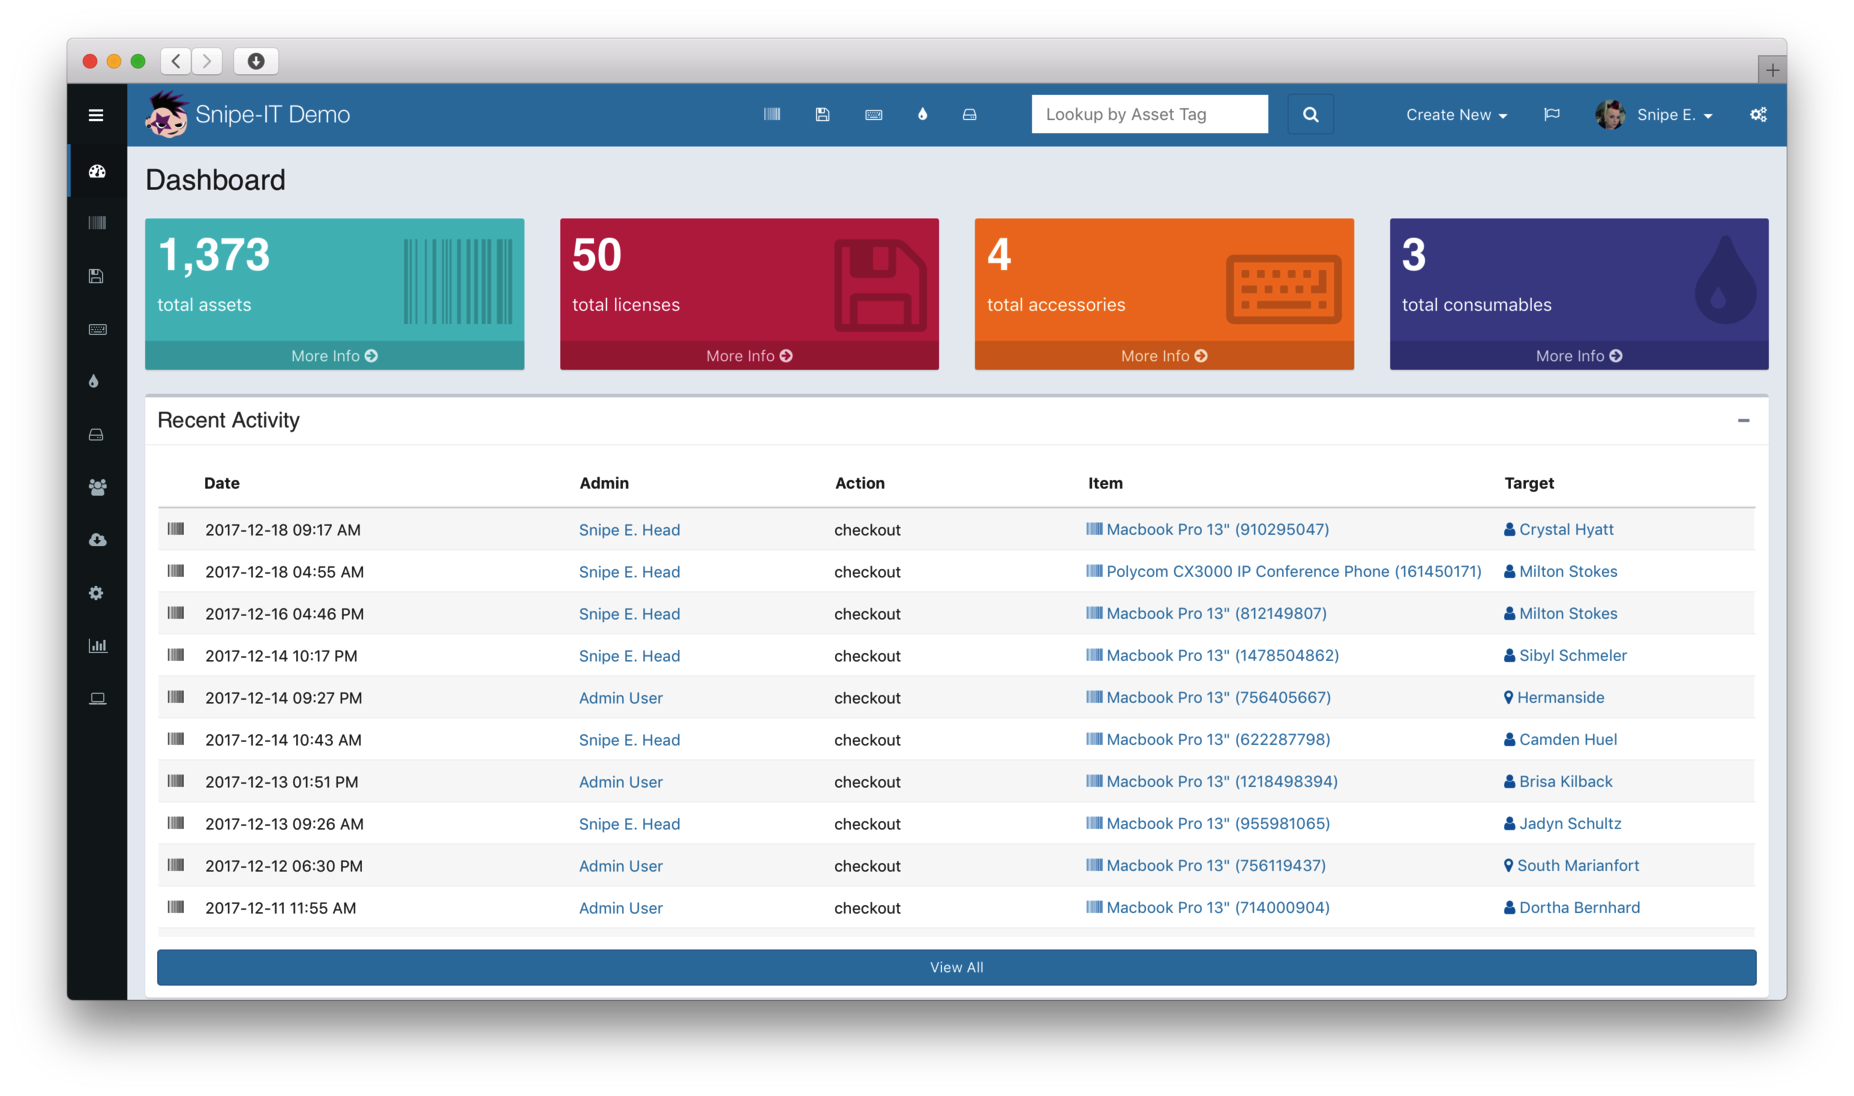
\includegraphics[width=\textwidth]
    {./graphics/snipe-dashboard.png}
    \caption{\label{fig:snipe-it-dashboard}Snip-IT dashboard waarin we het totale aantal assets binnen de organisatie kunnen zien, alsook een oplijsting van verschillende toestellen recent toegekend zijn~\autocite{snipe-it-dashboard}.}
\end{figure}

De software biedt een gebruiksvriendelijke webinterface (\ref{fig:snipe-it-dashboard}) waarmee bedrijfsmiddelen, licenties, garanties en meer gemakkelijk kunnen worden beheerd.
Wanneer men kiest voor de self-hosted optie is de software gratis beschikbaar, terwijl ook verschillende cloud-gebaseerde optie beschikbaar zijn tegen een jaarlijkse bijdrage.
Deze prijs varieert afhankelijk van de nodige features en support.
Alle code en services gerelateerd aan Snipe-IT zijn vrij beschikbaar op GitHub~\autocite{snipe-it-github}.

Enkele van de belangrijkste functies van Snipe-IT zijn~\autocite{snipe-it-features}, maar zijn niet beperkt tot:
\begin{itemize}
    \item Gemakkelijk zien welke assets zijn toegewezen, aan wie, en hun fysieke locatie
    \item In één klik inchecken
    \item Assetmodellen waarmee je gemeenschappelijke functies kunt groeperen
    \item Vereisen van Gebruikersacceptatie (Eindgebruikers EULA's/Gebruiksvoorwaar-\ den) bij Uitchecken
    \item E-mailmeldingen voor het verlopen van garanties en licenties
    \item Integratie met de meeste handheld barcode scanners en QR-codelezer apps
    \item Snelle en eenvoudige asset-audit
    \item Voeg je eigen aangepaste velden toe voor extra assetattributen
    \item Assets gemakkelijk importeren en exporteren
    \item Genereer QR-code labels voor eenvoudige mobiele toegang en labeling
    \item Assets gemarkeerd als aanvraagbaar kunnen worden aangevraagd door een gebruiker
    \item Assets behouden een volledige geschiedenis inclusief uitchecken, inchecken en onderhoud
    \item Optionele digitale handtekeningen bij assetacceptatie
\end{itemize}

\subsection{Lansweeper}
\label{sub:lansweeper}

Lansweeper, opgericht in 2004, is een Belgisch commercieel IT discovery \& inventory platform~\autocite{lansweeper-history}.
Het is een veelgebruikte tool voor het scannen, bijhouden en beheren van IT-assets binnen een organisatie.
Met functionaliteiten voor zowel hardware- als software-inventarisatie, biedt Lansweeper gebruikers een uitgebreid overzicht van alle IT-assets in hun netwerk.

Het grote voordeel van Lansweeper ten opzichte van andere tools, zoals Snipe-IT, is dat het een volledig geautomatiseerde oplossing biedt~\autocite{lansweeper-features}.
Dit betekent dat het platform in staat is om automatisch alle IT-assets binnen een netwerk te detecteren, zonder handmatige configuratie of de noodzaak om op elk systeem een agent te installeren~\autocite{lansweeper-getting-started}.
Een scan zal essenti\"ele informatie verzamelen over het asset, zoals de versie van het besturingssysteem, de hostname van de machine, het MAC-adres en de laatst ingelogde gebruiker.
Dit gebeurt met behulp van verschillende protocollen, waaronder SNMP.
De gedetecteerde informatie wordt vervolgens opgeslagen in een centrale database en is toegankelijk via een gebruiksvriendelijke webinterface.

\begin{figure}[h!]
    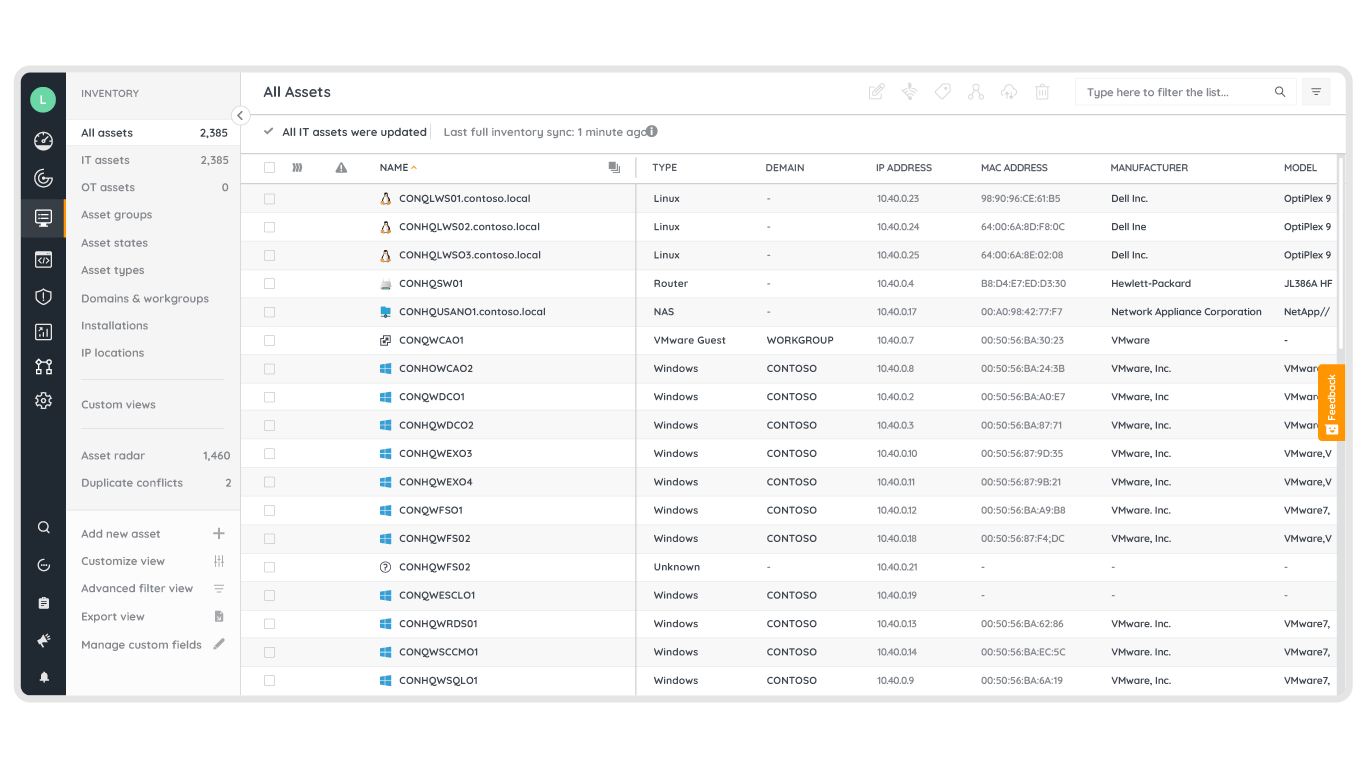
\includegraphics[width=\textwidth]
    {./graphics/lansweeper-dashboard.png}
    \caption{\label{fig:lansweeper-dashboard}Lansweeper dashboard waarin we een oplijsting van verschillende toestellen binnen de organisatie met basisinformatie over dat toestel, zoals: type, IP-adres en MAC-adres~\autocite{lansweeper-dashboard}.}
\end{figure}

Gebruikers kunnen aangepaste rapporten genereren over verschillende aspecten van hun IT-infrastructuur, zoals hardwareconfiguraties, softwarelicenties, patchniveaus en meer~\autocite{lansweeper-features}.
Deze rapporten zijn bruikbaar voor audits, nalevingscontroles en capaciteitsplanning.

Naast het genereren van rapporten en het identificeren van nieuwe IT-assets, biedt Lansweeper ook de mogelijkheid om rogue devices op het netwerk te detecteren.
Deze detectie gebeurt door continu het netwerk te scannen en alle gevonden assets te vergelijken met de resultaten in de database van bekende assets.
Wanneer een apparaat wordt gedetecteerd dat niet voorkomt in de database, genereert Lansweeper een waarschuwing, waardoor beheerders en administrators actie kunnen ondernemen.
Bovendien heeft Lansweeper de capaciteit om mogelijke beveiligingsrisico's te identificeren binnen uw inventaris door gebruik te maken van de NIST National Vulnerability Database~\autocite{lansweeper-cam}.
